\documentclass{beamer}
\usetheme{Madrid}
\usecolortheme{beaver}
\setbeameroption{hide notes}  % Notes are not shown.
% \setbeameroption{show notes}  % Notes are shown.
% \setbeameroption{show only notes}  % Only note pages are rendered.

% Set graphics location
\graphicspath{ {Images/} }

%Information to be included in the title page:
\title{Structural Quality \& Software Evolution}
\author{Alison Major}
\institute{Lewis University}
\date{2022}

% \logo{
%   
\includegraphics[width=0.2\textwidth]{UniversityLogo}
% }

\begin{document}

% =============================================================================

\frame{\titlepage}

% ----- Title Page Notes ------------------------------------------------------
\note{
  \begin{itemize}
    \item My name is Alison Major.
    \item I have researched the impact that the structural quality of software in open source Python projects can have on the evolution of the software.
  \end{itemize}
}

% =============================================================================

\begin{frame}
  \frametitle{Introduction}
  \textbf{Maintainability Index and Refactor Scores}
  \begin{itemize}
    \vspace{0.35cm}
    \item Areas of concern: cost, timeline, quality
    
    \vspace{0.35cm}
    \item Quality is hard to understand
    
    \vspace{0.35cm}
    \item Pylint \& Radon are a static analysis tools
    
    \vspace{0.35cm}
    \item Refactor violations point out code smells
  \end{itemize}
\end{frame}

% ----- Introduction Notes ----------------------------------------------------
\note{
  \begin{itemize}
    \item When we build new software solutions, there are several areas of concern.
    \item Namely, COST, TIME-TO-DELIVER, and also, often to a lesser extent, QUALITY.
    \item Though quality can be a factor we consider when planning a project, it is a hard characteristic to understand and measure.
    \item There are a number of tools available for enforcing standards, some built into IDEs (like Visual Studio Code) and others as 3rd party linter tools.
    \item Two such tools are Pylint and Radon, which can be used to analyze Python projects.
    \item In particular, we will focus on the REFACTOR violations that are noted in the code reports from Pylint and Radon, as these warnings can lead us to code smells.
  \end{itemize}
}

% =============================================================================

\begin{frame}
  \frametitle{Keeping Users Engaged Long Term}
  \textbf{Why does software evolution matter?}
  \begin{itemize}
    \item Users find bugs
    \item Users want new features
    \item New security threats
    \item New laws from governing bodies
  \end{itemize}
  
  \vspace{0.5cm}
  Need a thriving community of engaged users in order to keep apps and games successful.

  \vspace{0.35cm}
  In an open source system, need a thriving community of engaged developers in order to continue evolving.
\end{frame}

% ----- Keeping Users Engaged Notes -------------------------------------------
\note{
  \begin{itemize}
    \item Sometimes ``evolution'' is just a matter of maintenance and fixing bugs that users find.
    \item However, if users are engaged and actively using software, they are going to push the software to its limits and want new features.
    \item Over time, there can also be new security threats and new laws that require software to be updated.
    \item These different driving forces require a community of engaged users and in repsect to open source software, a community of engaged developers.
  \end{itemize}
}

% =============================================================================

\begin{frame}
  \frametitle{Keeping Users Engaged Long Term}
  \textbf{How do we ensure software evolution?}

  \vspace{0.35cm}
  Keep the project maintainable.
  \begin{itemize}
    \item Bugs should be quick and easy to fix
    \item New features should be easy to add
    \item Consistent standards (naming, small methods, etc)
  \end{itemize}

  \vspace{0.5cm}
  \textbf{Software Maintenance}
  \newline Large portion of project cost in a typical software system is in the maintenance phase.
\end{frame}

% ----- Keepign Users Engaged Pt. 2 Notes ------------------------------------
\note{
  \begin{itemize}
    \item So how do we make sure that our projects that we plan to build will evolve?
    \item We need to make sure the project stays maintainable.
    \begin{itemize}
      \item Bugs and new features should be easy to do
    \end{itemize}
    \item Part of what allows for easy changes is having consistent standards.
    \begin{itemize}
      \item Naming conventions
      \item Keeping methods small
      \item Having organized files
    \end{itemize}
    \item The majority of a typical project's cost lies not in the development phase, but in the maintenance phase!
    \item Maintenance is an important part of a software solution's lifecycle; we cannot ignore it!
  \end{itemize}
}

% ============================================================================

\begin{frame}
  \frametitle{The Impact of Structural Quality}
  \textbf{Measuring Maintainability}
  \begin{itemize}
    \vspace{0.35cm}
    \item Easy to maintain = Easy to evolve
    
    \vspace{0.35cm}
    \item Pylint \& Radon Maintainability Index (MI)

    \vspace{0.35cm}
    \item PEP 8 is a set of Python standards

    \vspace{0.35cm}
    \item Refactor Messages (Pylint)
    \begin{itemize}
      \item Refactor warnings are generally ``code smells''
      \item Code smells point out problems in Architecture
    \end{itemize}
  \end{itemize}
\end{frame}

% ----- Measuring Maintainability Notes ---------------------------------------
\note{
  \begin{itemize}
    \item So, if we want to keep our projects easy to maintain so that they are easy to evolve, how do we MEASURE that maintainability?
    \item Pylint and Radon are tools I mentioned earlier that provide a measurement known as the Maintainability Index.
    \item In Pylint's reports, they also provide a number of different messages:
    \newline Convention, Error, Fatal, Information, Refactor, Warning
    \item These types of messages are defined using PEP 8, which is a set of Python standards than can be used as a set of ``best practices''
    \item Today we focus on the refactor messages, as they will generally lead us to ``code smells'', which are problems in the software's architecture.
  \end{itemize}
}

% ============================================================================

\begin{frame}
  \frametitle{The Impact of Structural Quality}
  \textbf{Other Maintainability Characteristics}
  \begin{itemize}
    \vspace{0.35cm}
    \item Low coupling, high cohesion
    
    \vspace{0.35cm}
    \item Readability
    \begin{itemize}
      \item Big commits reduce maintainability
      \item PEP 8 enforces readability
    \end{itemize}
    
    \vspace{0.35cm}
    \item Confidence that metrics around software structure provide value in keeping systems maintainable (and therefore can evolve) % \cite{zhou:2020}
  \end{itemize}
\end{frame}

% ----- Other Maintainability Characteristics Notes ---------------------------
\note{
  \begin{itemize}
    \item Refactor warnings aren't the only only thing we should care about for good maintainability.
    \item We should also remember other good practices, like low coupling and high cohesion.
    \begin{itemize}
      \item Coupling refers to the degree to which different modules depend on each other (we want modules to be independent from each other)
      \item and cohesion refers to the degree in which elements of a module belong together (we want to bind related code together)
    \end{itemize}
    \item We also want good readability (big commits can be hard to follow)
    \item And having confidence around the metrics that tools like Pylint and Radon can offer should be able to help us keep our systems maintainable.
  \end{itemize}
}

% ============================================================================

\begin{frame}
  \frametitle{The Impact of Structural Quality}
  \textbf{Documentation and Maintainability}
  \begin{itemize}
    \vspace{0.35cm}
    \item Documentation holds the results of significant design decisions
    
    \vspace{0.35cm}
    \item Can influence the ability to evolve because\dots
    \begin{itemize}
      \item Enhances code understanding
      \item Comprehensibility impacts maintainability in a positive way  
    \end{itemize}
  \end{itemize}
\end{frame}

% ----- Documentation and Maintainability Notes ------------------------------
\note{
  \begin{itemize}
    \item To add to the ideas of maintainability and readable code, we should also remember that documentation can feed into our success.
    \item When we build a software system, good documentation can hold significant design decisions.
    \item This ``historical record'' can help developers in the open source community understand the code and why things are the way they are.
    \item Better comprehension makes it easier to maintain and evolve the code.
  \end{itemize}
}

% ============================================================================

\begin{frame}
  \frametitle{Related Work}
  \textbf{Design Patterns and Software Quality}
  \begin{itemize}
    \vspace{0.35cm}
    \item Design patterns provide flexibility
    
    \vspace{0.35cm}
    \item Classes with frequent changes are either...
    \begin{itemize}
      \vspace{0.15cm} 
      \item Easy to extend (okay)
      \vspace{0.15cm} 
      \newline ...or...
      \vspace{0.15cm}
      \item Correlate to other classes (high coupling... red flag!)
    \end{itemize}
    
    \vspace{0.35cm}
    \item We look at refactor score (code smell) not error score (bugs)
  \end{itemize}
  
  \vspace{0.35cm}
  Keeping this in mind, we focus on \emph{changes for system extensions and adaptiation}, not bug fixes.
\end{frame}

% ----- Design Patterns & Software Quality Notes ------------------------------
\note{
  \begin{itemize}
    \item Through our studies, we also know that design patterns can lead us to better ways to build our code, which provides us with more flexibility.
    \item As we review open source systems, finding code classes with frequent changes generally mean one of two things\dots
    \begin{itemize}
      \item the class is easy to extend (which is good!)
      \item or the class is highly coupled to other classes which means updating one requires updates to another (code smell!)
    \end{itemize}
    \item Keeping this in mind, we again are reminded to steer towards understanding the frequency of refactor messages, or code smells, over error scores, which are just bugs and not an indicator of how maintainable the code is.
  \end{itemize}
}

% ============================================================================

\begin{frame}
  \frametitle{Related Work}
  \textbf{Software Architecture and Maintainability}
  \begin{itemize}
    \vspace{0.35cm}
    \item Maintainability
    
    \vspace{0.35cm}
    \item Extensibility
    
    \vspace{0.35cm}
    \item Simplicity, understanding
    
    \vspace{0.35cm}
    \item Re-usability
    
    \vspace{0.35cm}
    \item Performance
  \end{itemize}

  \vspace{0.35cm}
  {\small \emph{Keep these in mind for easier future development when adding or changing code.}}
\end{frame}

% ----- Related Work Notes ----------------------------------------------------
\note{
  \begin{itemize}
    \item With all of these attributes and characteristics we've discussed, we can boil a lot of this down to the product quality model that the committee of the International Organization for Standardization and the International Electrotechnical Commission has provided us with:
    \begin{itemize}
      \item Maintainability (our topic of interest)
      \item Extensibility
      \item Keeping things simple
      \item Keeping things reusable
      \item Focusing on performance 
      \item etc.
    \end{itemize}
    \item Helping developers keep these in mind when adding or changing code will allow for easier FUTURE development.
  \end{itemize}
}

% ============================================================================

\begin{frame}
  \frametitle{Methodology}
  \textbf{Initial Repository Set}
  \begin{itemize}
    \item Popular
    \item Long development history
    \item Multiple release cycles
  \end{itemize}

  \vspace{0.35cm}
  \textbf{Filtered Respository Set}
  
  \emph{At least 80\% Python code and top 20th percentile in these categories:}
  \begin{itemize}
    \item Long history of commits (2,968+ commits)
    \item Large number of contributors (90+ contributors)
    \item Many releases (44+ releases)
    \item Substantial Age (66.4+ months)
  \end{itemize}

  \vspace{0.35cm}
  Results in 46 repositories for further research.
\end{frame}

% ----- Methodology Notes -----------------------------------------------------
\note{
  \begin{itemize}
    \item Now we're ready for the data!
    \item We started with a larger set of open source python projects on GitHub that were popular (lots of stars), had a long commit history, and contained multiple release cycles.
    \item From there, we filtered the set down to any projects that contained at least 80\% Python code.
    \item And finally, we found the top 20th percentile in several key categories.
    \item This left us with 46 repositories for deeper study.
  \end{itemize}
}

% ============================================================================

\begin{frame}
  \frametitle{Results}
  \begin{itemize}
    \item Radon MI for all repositories rank as grade ``A''
    \newline which is considered ``very high maintainability''
    \item Open source systems with engaged community 
    \newline of developers tend to have higher scores
    \item For comparison, calculated ratio of refactor message count 
    \newline to SLOC as well as the average MI for a project.
  \end{itemize}

  \vspace{0.25cm}
  \begin{center}
    \begin{tabular}{ c c c c }
      \textbf{Repo} & \textbf{Ratio} & \textbf{Avg MI} & \textbf{Status} \\ 
      \hline\hline
      cython & 0.14 & 31.0 & active \\ \hline  % Best
      youtube-dl & 0.15 & 54.16 & active \\ \hline  % 2nd Best
      electrum & 0.16 & 39.41 & active \\ \hline  % 3rd Best
      \hline
      numba & 0.62 & 62.55 & active \\ \hline  % 3rd Worst
      scrapy & 0.64 & 64.47 & active \\ \hline  % 2nd Worst
      raven-python & 1.35 & 87.02 & deprecated \\ \hline  % Worst
    \end{tabular}
  \end{center}
\end{frame}

% ----- Results Notes ---------------------------------------------------------
\note{
  \begin{itemize}
    \item With our smaller data set on hand, we ran Radon against each repository to gain a Maintainability Index.
    \item For a very simplified view, we averaged the Maintainability Index of each project files, giving us a single number for general comparison with each repository.
    \item In Radon's grading system, any value over 20 is considered ``very maintainable'' code.
    \item We also used a count of the Pylint REFACTOR messages and calculated the ratio of messages to source-line-of-code for an idea of how many code smells each project contained, relative to its size.
    \item Listed in the table are the ``best 3'' (cython, youtube-dl, and electrum) and the ``worst 3'' (raven-python, scrapy, and numba) in regards to their refactor ratios.
  \end{itemize}
}

% ============================================================================

\begin{frame}
  \frametitle{Results}
  \begin{center}
    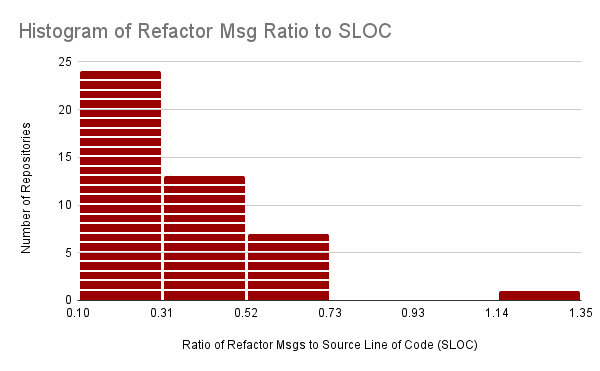
\includegraphics[width=0.8\columnwidth]{Histogram of Refactor Msg Ratio to SLOC.png}
  \end{center}
  \begin{center}
    {\small \emph{Diligent development communities can keep refactor warnings low,}}
    
    {\small \emph{regardless of system size (lines of code).}}
  \end{center}
\end{frame}

% ----- Results Pt. 2 Notes ---------------------------------------------------
\note{
  \begin{itemize}
    \item With this information, we can get an idea of where these projects stand in regards to their refactor message ratios compared to each other.
    \item This histogram shows that the majority of our repository set have a very low ratio of refactor messages.
    \item This could indicate that our projects are all highly maintainable.
    \item This may be a impacted by the data set we chose; perhaps projects with highly engaged communities tend to keep their code in a maintainable state, because this would be the only way for many people to be involved.
  \end{itemize}
}

% ============================================================================

\begin{frame}
  \frametitle{Results}
  \begin{center}
    % 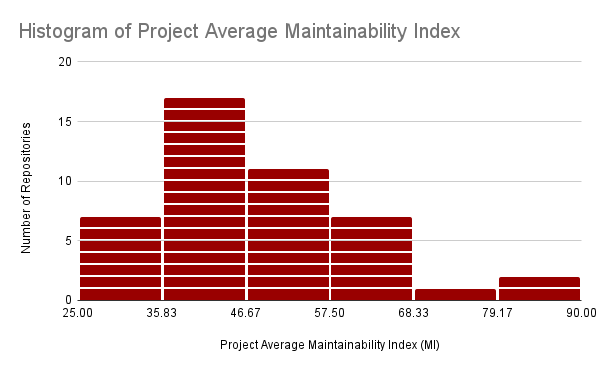
\includegraphics[width=0.8\columnwidth]{Histogram of Project Average Maintainability Index.png}
    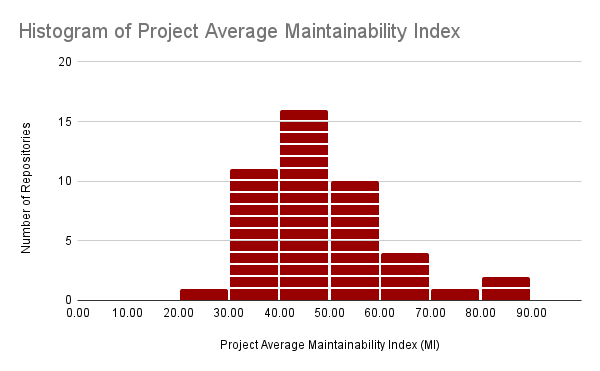
\includegraphics[width=0.8\columnwidth]{Histogram of Project Average Maintainability Index_BucketSize_10.png}
  \end{center}
  \begin{center}
    {\small \emph{Many repositories average in the mid-score to high-score.}} 
    
    {\small \emph{Radon considers 20 points and up to be very maintainable.}}
  \end{center}
\end{frame}

% ----- Results Pt. 3 Notes ---------------------------------------------------
\note{
  \begin{itemize}
    \item To view the same repository set with their Maintainability Index averages, we have another histogram.
    \item This score can range from 0 (awful) to 100 (perfect).
    \item Remember that Radon considers any value above 20 to be an ``A'' or ``very maintainable''.
    \item We can see that all of our projects receive an ``A'' grade, with the majority in the middle of the range, which can be from zero to 100.
  \end{itemize}
}

% ============================================================================

\begin{frame}
  \frametitle{Conclusions}
  \begin{itemize}
    \item Structural quality impacts software evolution.
    
    \vspace{0.35cm}
    \item Good projects will grow and evolve.
    
    \vspace{0.35cm}
    \item Poor structure leads to deprecation.
    \begin{itemize}
      \item If the development community is engaged, deprecation of 
        \newline the project may lead to a fresh, improved code base.
    \end{itemize}
    
    \vspace{0.35cm}
    \item Open source and projects with many contributors are vulnerable to degrading maintainability.
    \begin{itemize}
      \item Popular repositories with a long history of commits and releases 
        \newline (i.e. our repository data set) tend to have good maintainability.
      \item The high maintainability is a testament to their longevity.
    \end{itemize}
  \end{itemize}
\end{frame}

% ----- Conclusions Notes -----------------------------------------------------
\note{
  \begin{itemize}
    \item Our very best and very worst repositories are all still actively being improved and evolving, even today.
    \item An exception to this is our ``worst'' repository, raven-python, which was deprecated, but in exchange for an improved system.
    \item It didn't actually die, but the community recognized that a better architecture was needed for the system to continue to evolve.
    \item Open source systems, and any project with many contributors or many changes are vulnerable to degrading quality. It's the nature of change over time.
    \item However, when we review a set of popular repositories that already have a long history of commits, we find that they tend to have good maintainability.
  \end{itemize}
}

% ============================================================================

\begin{frame}
  \frametitle{Recommendations}
  \begin{itemize}
    \item Good architecture is important for evolution.
    
    \vspace{0.35cm}    
    \item Reliable quality metric can be a useful way to measure maintainability, which promotes ability to evolve a project.
    
    \vspace{0.35cm}
    \item Pick a set of standards to maintain good architecture 
    \newline even with a large, open source community.
    \begin{itemize}
      \item Limit complexity as project changes and grows.
      \item SOLID principles.
      \item Keep it DRY.
      \item And other design patterns known to be best practice.
    \end{itemize}
    
    \vspace{0.35cm}
    \item Auto-enforce by using quality measurements for desired standards 
    \newline in the project's CI/CD pipeline.
  \end{itemize}
\end{frame}

% ----- Recommendations Notes -------------------------------------------------
\note{
  \begin{itemize}
    \item Where do we go from here?
    \item In regards to the data, we'd like to do more study to understand the correlation between the Pylint metrics and Maintainability Index in order to gain further insight.
    \item What we've found so far is a reinforcement of what many of us already know.
    \item Good architecture is important for software to evolve.
    \item Reliable quality metrics can be helpful to keep an architecture ready for enhancements.
    \item Regardless of your code base, your team should understand what set of standards will work best for your software solution.
    \item Then auto-enforce these standards in your pipeline. This keeps everyone honest and will improve the ability to evolve your project.
    \item Thank you for your time and attention!
    \item Any questions?
  \end{itemize}
}

% ============================================================================

\end{document}